%\newcommand{\beginsupplement}{%
%\setcounter{table}{0}
%\renewcommand{\thetable}{S\arabic{table}}%
%\setcounter{figure}{0}
%\renewcommand{\thefigure}{S\arabic{figure}}%
%\setcounter{equation}{0}
%\renewcommand{\theequation}{S\arabic{equation}}%
%}
%\beginsupplement
%\makeatletter
%\makeatother

\chapter[Supplementary information for "Dielectric surface loss in superconducting resonators with flux-trapping holes"]{Supplementary information for "Dielectric surface loss in superconducting resonators with flux-trapping holes"}
\label{ch:Vortex-supp}

%\begin{center}
    %\textbf{Supplementary information for "Dielectric surface loss in superconducting resonators with flux-trapping holes"}
%\end{center}

\def \Bcapp {\text{B}^{\text{cool}}_{\text{applied}}}

We show the data and analysis estimating residual magnetic loss in superconducting resonators with flux-trapping hole arrays. We describe the design rules used to embed a meandered resonator in a rectangular array of holes.  We show data supporting the claim that the maximum in $Q_{i}$ is obtained at an applied magnetic field that cancels the ambient field.  We report the TLS model parameters for resonators from the MBE and ebeam deposited films from which we estimate the excess loss attributable directly to the densest hole pattern.
% \maketitle
\section{quality factor extraction}
In the main text, we infer resonator loss 1/$Q_i$ by measuring the system scattering parameters (S-parameters) of superconducting coplanar waveguide (SCPW) resonators capacitively coupled to a feedline.  The circuit model for this system has been analysed previously \cite{megrant2012} and gives the result
\begin{equation}
    \label{spectroscopyS21}
    \tilde{S}_{21}^{-1} = 1 + \frac{Q_{i}}{Q_{c}^{*}}e^{i \phi}\frac{1}{1+i2 Q_{i} \frac{f-f_{0}}{f_{0}}}
\end{equation}
Here $\tilde{S}_{21}^{-1}$ is the inverse of transmission data calibrated to enforce $S_{21}=1$ far off resonance.  $f_{0}$ and $\phi$ are the resonant frequency and impedance mismatch angle and  $Q_{c}^{*}$ is the coupling quality factor scaled by an impedance ratio.

\begin{figure}[b]
    \begin{center}
        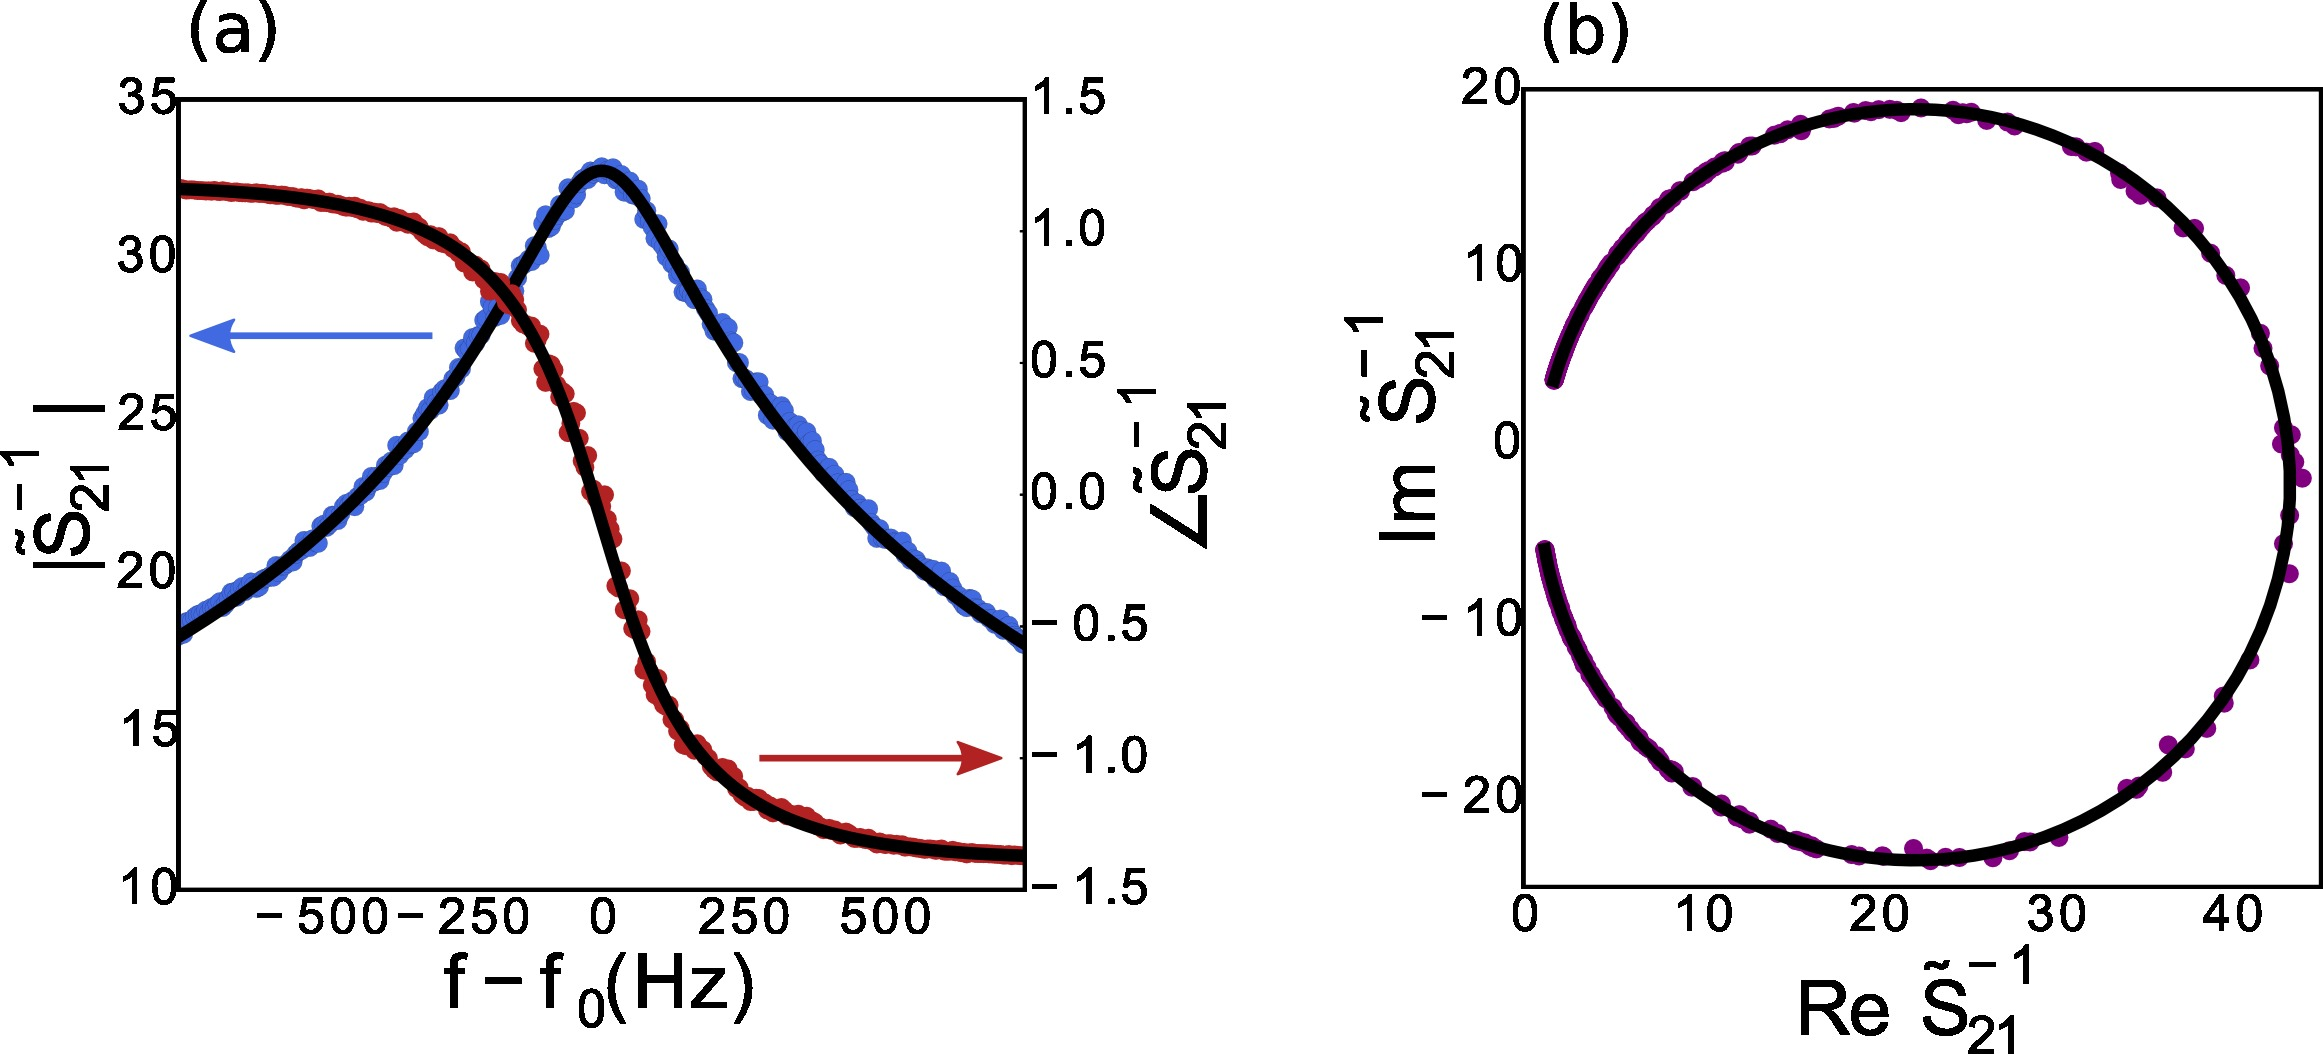
\includegraphics[width=150mm]{DielectricFluxTrap_Supp_Rev2_basicfit.jpg}
        \caption{(Color online)  The transmission spectroscopy data for the extraction of $Q_{i}$ shown as (a) magnitude and phase and (b) in the complex plane.}
        \label{basicfit}
    \end{center}
\end{figure}
%\newpage

We extract the internal quality factor $Q_{i}$ and its statistical uncertainty $\sigma_{Q_{i}}$ by fitting measurements of our device to this model.  Figure \ref{spectroscopyS21} shows example data from the MBE sample for which the $Q_{i} = 1.86 \times 10^{7} \pm 2.58 \times 10^{5}$.  This is representative of the data points shown in Fig\,\ref{novortexdata}.

\section{Residual magnetic loss}
Fig.\,\ref{novortexdata} breaks out the data in Fig.\,2a of the main text for resonators with ground plane holes from the MBE sample in the region from $\Bcapp$ = 1.4\,$\mu T$ to 6.4\,$\mu T$.  This is below the critical field for vortex formation in both the center trace of the resonator and in the ground plane near the resonator where there are ground plane holes.  Thus, we do not expect magnetic loss in this region.  In Fig.\,\ref{novortexdata} we apply a linear loss model $1/Q_{i}$\,=\,$m$\,$\times$\,$\Bcapp$\,+\,$b$ to the data and obtain the parameters m and b with a weighted least squares fit.  We use weighting factors $1/\sigma^2_{\left( 1/Q_i \right)}$, where $\sigma_{\left( 1/Q_i \right)}=\left( -1/Q_{i}^{2} \right) \sigma_{Q_{i}}$ in terms of parameters extracted directly from device data.  We obtain our estimate of residual magnetic loss from the parameter $m$ in these fits.  This estimate is $m = 8.6\times10^{-10} \pm 1.3\times 10^{-10}$ /$\mu T$, where the uncertainty represents the standard error.


\begin{figure}
    \begin{center}
        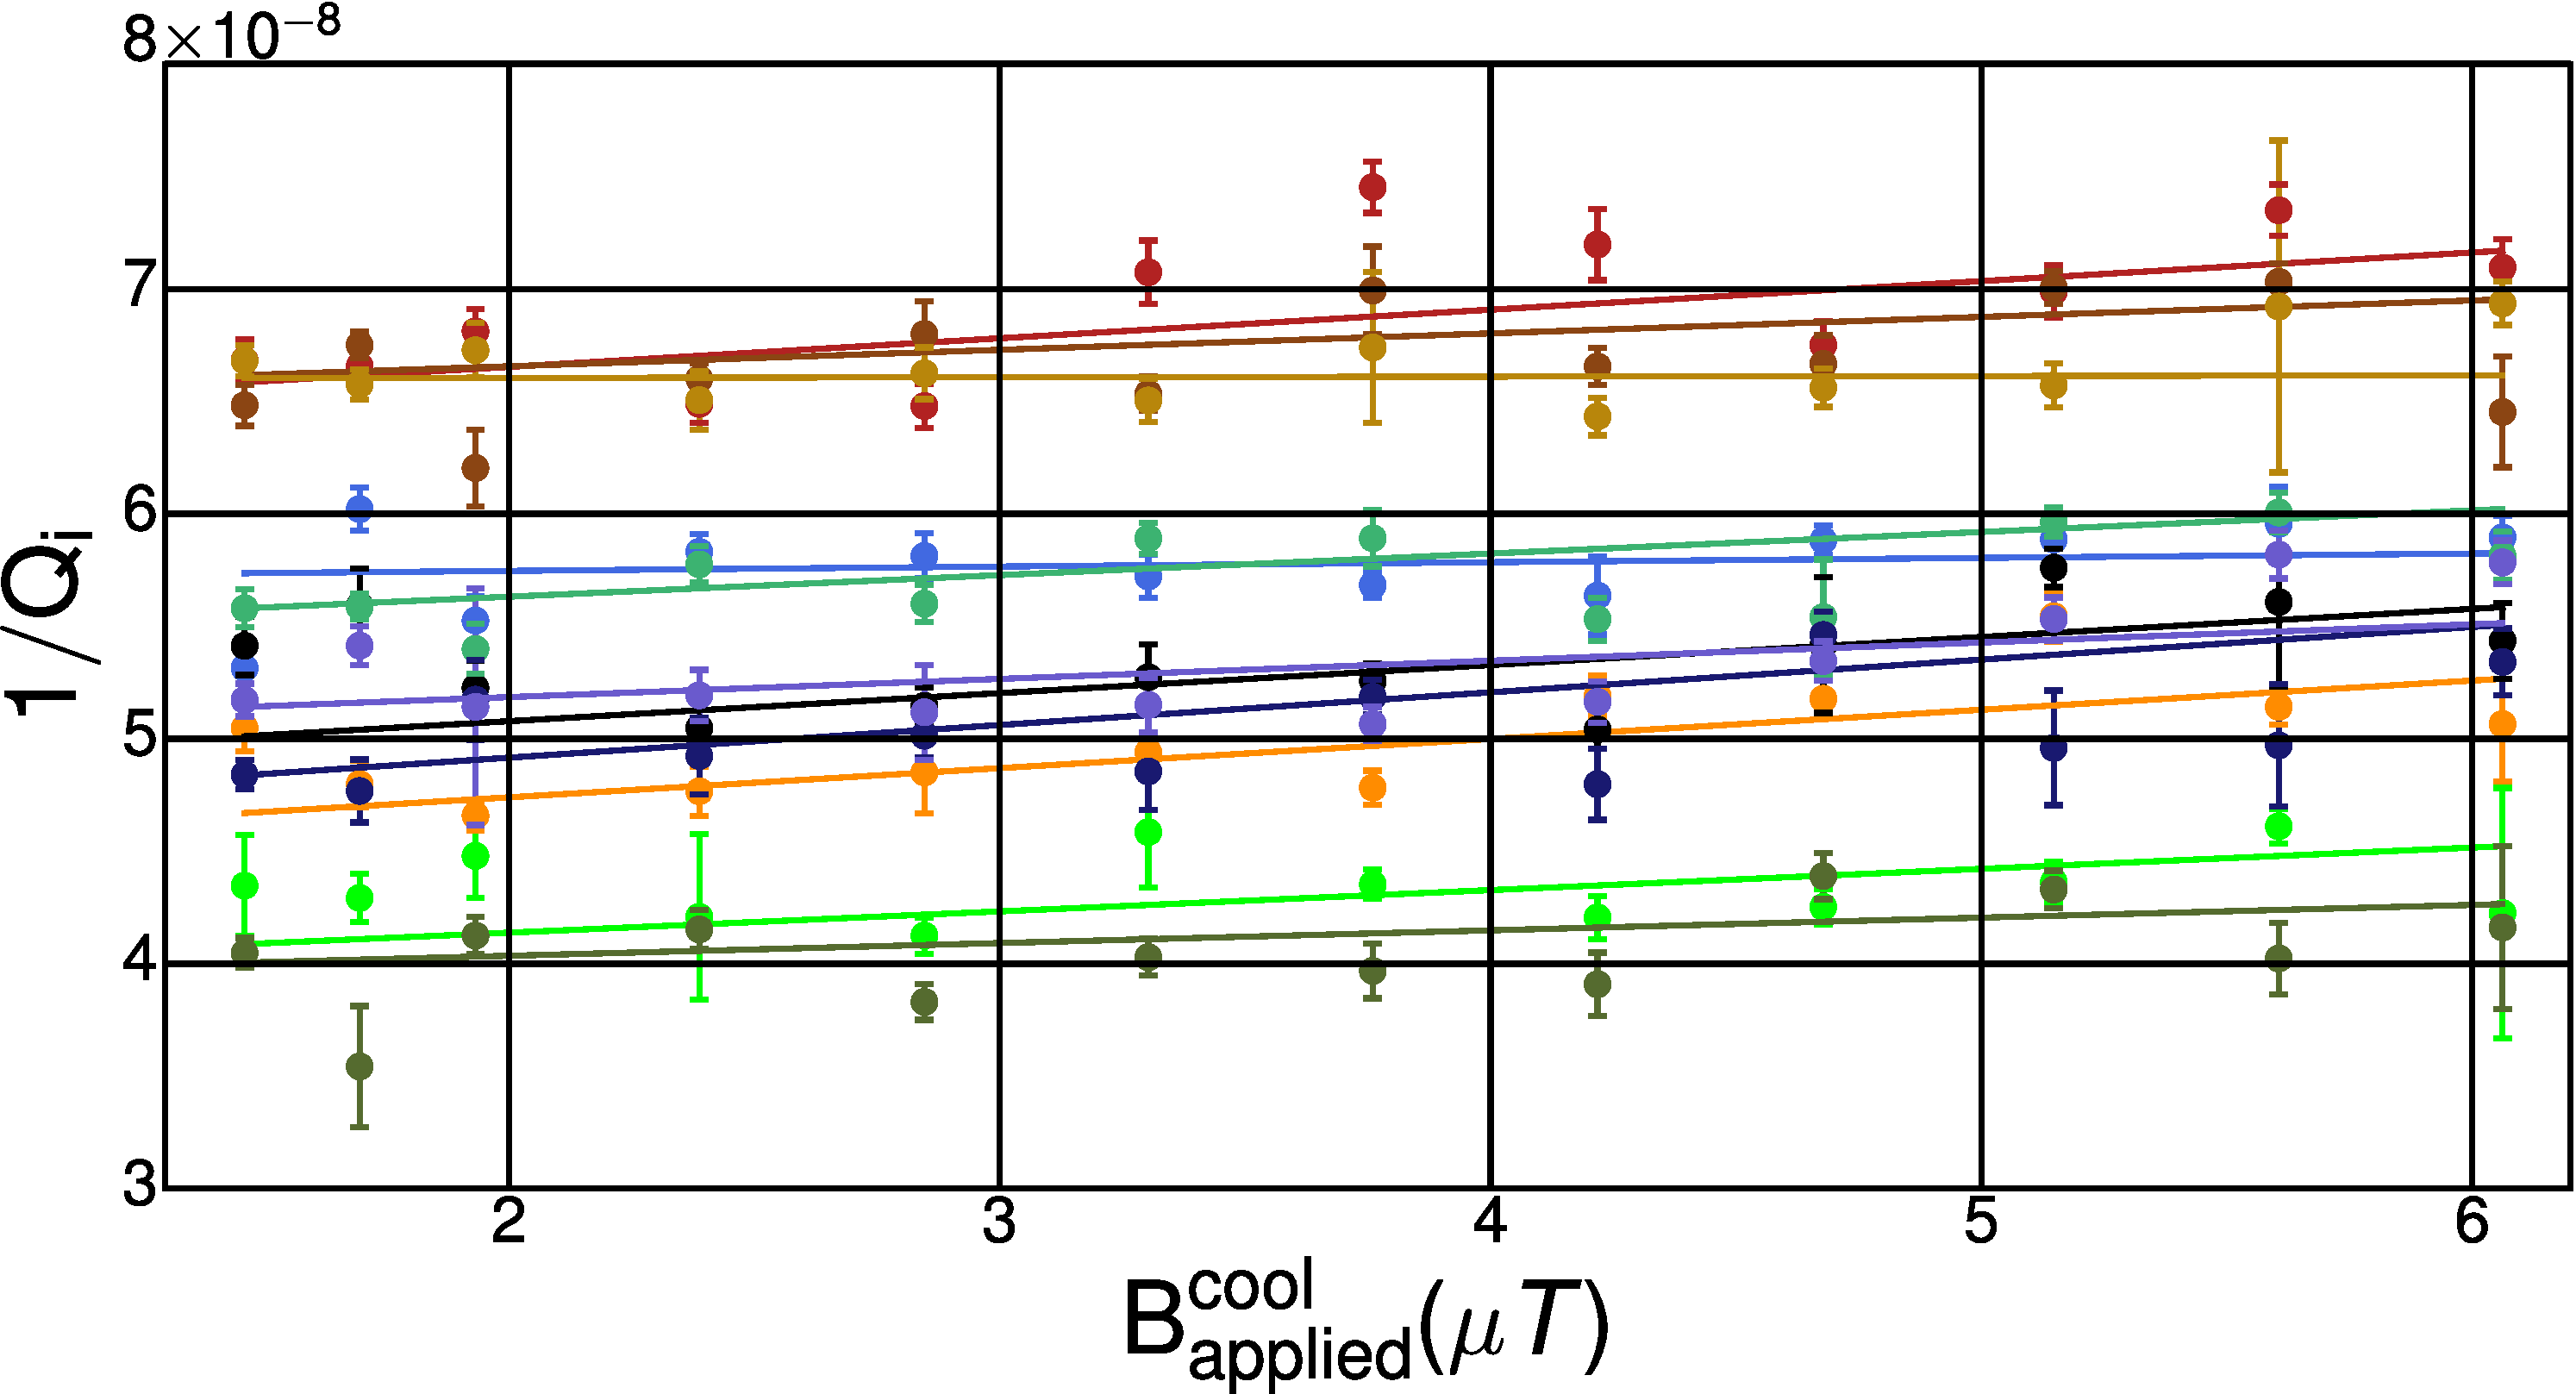
\includegraphics[width=150mm]{DielectricFluxTrap_Supp_Rev2_qnovortex.pdf}
        \caption{(Color)  The small magnetic field dependence of internal loss for 11 resonators with ground plane hole arrays.}
        \label{novortexdata}
    \end{center}
\end{figure}


\section{Hole pattern design rules}
In the main text, we describe the hole pattern as having a constant distance between the edges of adjacent holes and between the resonator edge and the nearest hole.  However, the curved portion of our meandered resonator geometry does not allow us to easily satisfy both of these constraints simultaneously.  We expect that excess dielectric loss from hole patterns will be primarily determined by the resonator edge to hole edge distance and dominated by the row of holes nearest the resonator edge.  The compromise that we have adopted is to have two rows of holes follow the contour of the resonator with a constant spacing between adjacent holes and the resonator edge.  This composite structure is then embedded in a rectangular array of regularly spaced holes.  An example is shown in fig. \ref{meander_holearray}.  This allows us to maintain a constant resonator to hole edge distance for the entire length of the resonator.
\begin{figure}
    \begin{center}
        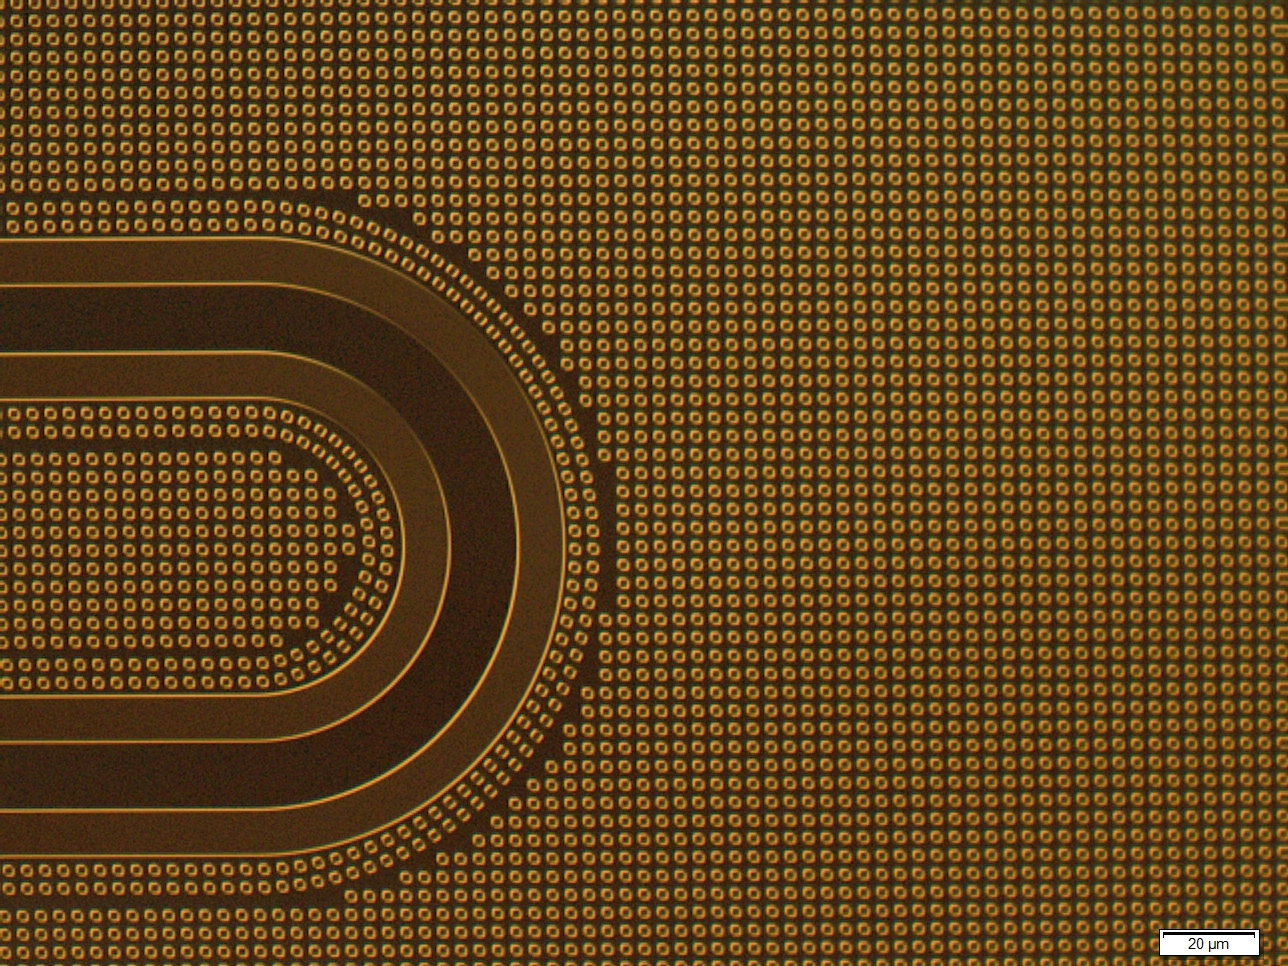
\includegraphics[width=150mm]{DielectricFluxTrap_Supp_Rev2_meander}
        \caption{The meandered section of a $\lambda$/4 resonator with a flux trapping holes showing two rows holes following the contour of the meander and the rectangular array of holes in which the resonator is embedded.}
        \label{meander_holearray}
    \end{center}
\end{figure}
%As the origin of this loss has not been determined, we claim this as an upper bound on the residual magnetic loss in superconducting resonators that have their ground plane patterned with flux-trapping holes.

In the main text, we claim that the maximum in $Q_i$ is obtained at an applied magnetic field that cancels the ambient field.  If the $Q_i$ maximum were due to vortex mediated quasiparticle recombination\cite{nsanzineza2014} rather than field cancellation then we would expect to observe a second maximum at a symmetric, negative magnetic field.   Fig\,\ref{fullfield} shows the field dependence of $Q_i$ at both positive and negative fields for four resonators without flux-trapping holes on one circuit from the ebeam deposited film.  The absence of a second maximum at negative fields shows that vortex mediated quasiparticle recombination does not play an important role in determining $Q_{i}$ in our system.  This is expected because our cryostat features extensive shielding and filtering to reduce the number of nonequilibrium quasiparticles and we operate the resonators well below $T_c$ so that the number of thermal quasiparticles is also small.

\begin{figure}
    \begin{center}
        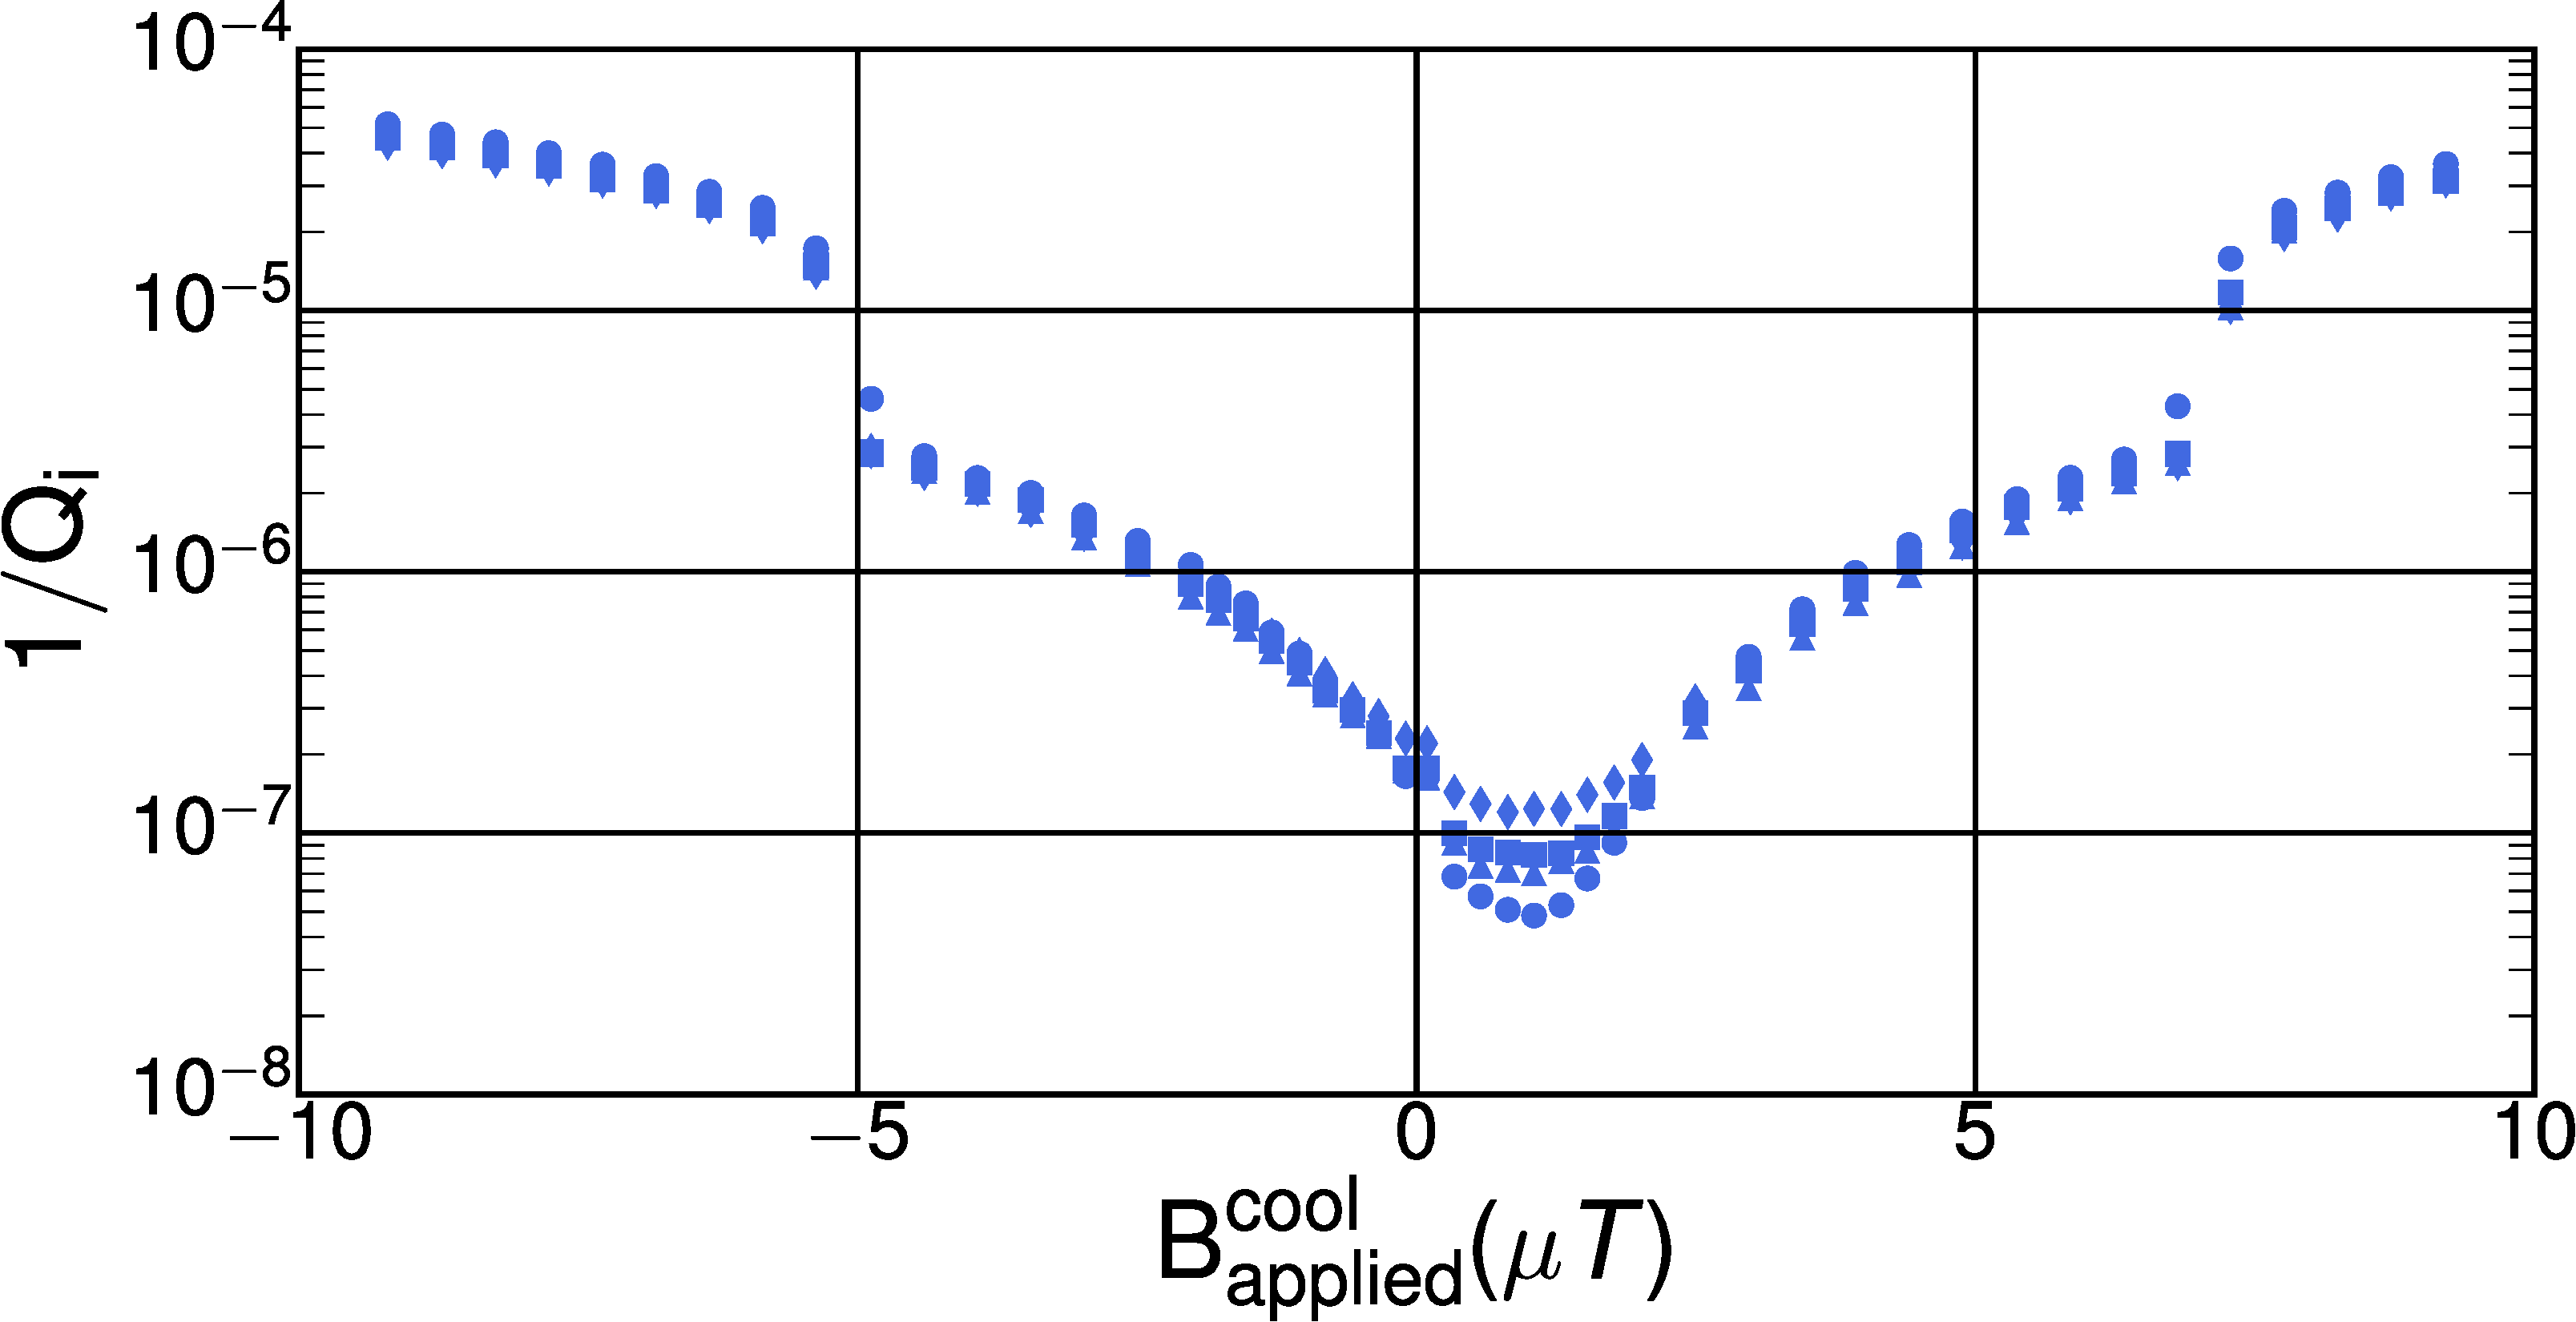
\includegraphics[width=150mm]{DielectricFluxTrap_Supp_Rev2_fullfield.pdf}
        \caption{The full field dependence of $Q_i$ for four resonators without flux-trapping holes from the ebeam deposited film.  The single loss minimum is observed when the total magnetic field is zero.}
        \label{fullfield}
    \end{center}
\end{figure}

\section{Dielectric loss estimate}
In the main text, we claim that the TLS loss due to the densest hole pattern is $2.5 \pm 1.3\times 10^{-7}$.  This claim is derived from measurements of 23 resonators summarized in table \ref{table:ResonatorData}.  We use the R statistics package\cite{R} to apply a linear regression to this data set, accounting for both the deposition technique and the hole pattern.  No interaction term was included in this model because the interaction between hole pattern and deposition technique was found to be statistically insignificant.  This analysis yields an estimate for TLS loss due to the dense hole pattern, the standard error of that estimated value, and a p-value indicating the statistical significance of this finding.  Those values were respectively $2.5\times10^{-7}$, $1.3\times10^{-7}$, and 0.07.

\begin{table}
    \caption{Deposition condition, hole density, and TLS model parameters extracted from the power dependence at $\Bcapp$ = 0}
    \centering
    \begin{tabular}{ c c c c c c}
        \hline \hline
        Deposition & 1/d $(\mu m^{-1})$ & $1/\text{Q}_{\text{tls}}$ & $1/\text{Q}_{0}$ & $\text{N}_{\text{sat}}$ & $\alpha$ \\
        \hline
        MBE & 0 & 7.3e-07 & 3.55e-08 & 21.8 & 0.81 \\
        MBE & 0 & 6.59e-07 & 4.92e-08 & 35.4 & 0.73 \\
        MBE & 0 & 1.19e-06 & 5e-08 & 10.7 & 0.71 \\
        MBE & 0 & 7.44e-07 & 5.82e-08 & 71.3 & 0.73 \\
        MBE & 0 & 7.3e-07 & 3.32e-08 & 54.1 & 0.82 \\
        MBE & 0 & 8.73e-07 & 4.44e-08 & 34.1 & 0.79 \\
        MBE & 0 & 9.4e-07 & 6.64e-08 & 52.7 & 0.75 \\
        MBE & 0.5 & 8.9e-07 & 4.01e-08 & 24.6 & 0.71 \\
        MBE & 0.5 & 9.26e-07 & 5.29e-08 & 16.4 & 0.68 \\
        MBE & 0.5 & 1.03e-06 & 4.23e-08 & 39.1 & 0.81 \\
        MBE & 0.5 & 1.56e-06 & 5.35e-08 & 36.4 & 0.86 \\
        ebeam & 0 & 1.1e-06 & 3.77e-08 & 20.1 & 0.75 \\
        ebeam & 0 & 1.26e-06 & 5.61e-08 & 9.7 & 0.69 \\
        ebeam & 0 & 1.2e-06 & 7.21e-08 & 34.8 & 0.74 \\
        ebeam & 0 & 1.63e-06 & 8.55e-08 & 37.3 & 0.80 \\
        ebeam & 0 & 1.88e-06 & 4.18e-08 & 8.0 & 0.78 \\
        ebeam & 0 & 1.23e-06 & 5.24e-08 & 10.6 & 0.64 \\
        ebeam & 0 & 1.63e-06 & 5.92e-08 & 20.5 & 0.70 \\
        ebeam & 0 & 1.18e-06 & 8.75e-08 & 30.5 & 0.61 \\
        ebeam & 0.5 & 1.06e-06 & 5.25e-08 & 50.8 & 0.82 \\
        ebeam & 0.5 & 1.54e-06 & 7.52e-08 & 30.8 & 0.80 \\
        ebeam & 0.5 & 1.55e-06 & 5.06e-08 & 25.8 & 0.74 \\
        ebeam & 0.5 & 2.3e-06 & 7.83e-08 & 12.6 & 0.77 \\
        \hline
    \end{tabular}
    \label{table:ResonatorData}
\end{table}
